\documentclass[12pt]{article}
\usepackage{tikz}
\usepackage{ctable}
\title{Draw Block Documentation}
\author{Jake Humphrey}
\begin{document}
\maketitle
\section{Finite State Machine}
\begin{center}
  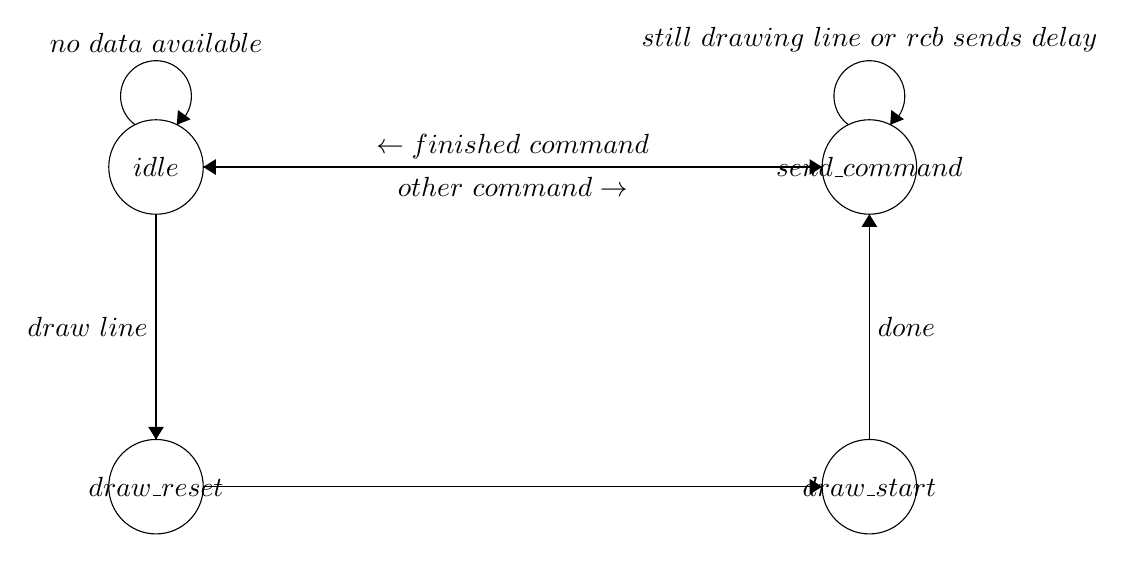
\begin{tikzpicture}[scale=0.2]
    \tikzstyle{every node}+=[inner sep=0pt]
    \draw [black] (18.1,-19.4) circle (3);
    \draw (18.1,-19.4) node {$idle$};
    \draw [black] (18.1,-39.7) circle (3);
    \draw (18.1,-39.7) node {$draw\_reset$};
    \draw [black] (63.4,-39.7) circle (3);
    \draw (63.4,-39.7) node {$draw\_start$};
    \draw [black] (63.4,-19.4) circle (3);
    \draw (63.4,-19.4) node {$send\_command$};
    \draw [black] (18.1,-22.4) -- (18.1,-36.7);
    \fill [black] (18.1,-36.7) -- (18.6,-35.9) -- (17.6,-35.9);
    \draw (17.6,-29.55) node [left] {$draw\mbox{ }line$};
    \draw [black] (21.1,-39.7) -- (60.4,-39.7);
    \fill [black] (60.4,-39.7) -- (59.6,-39.2) -- (59.6,-40.2);
    \draw [black] (63.4,-36.7) -- (63.4,-22.4);
    \fill [black] (63.4,-22.4) -- (62.9,-23.2) -- (63.9,-23.2);
    \draw (63.9,-29.55) node [right] {$done$};
    \draw [black] (60.4,-19.4) -- (21.1,-19.4);
    \fill [black] (21.1,-19.4) -- (21.9,-19.9) -- (21.9,-18.9);
    \draw (40.75,-18.9) node [above] {$\leftarrow finished\mbox{ }command$};
    \draw (40.75,-20.0) node [below] {$other\mbox{ }command \rightarrow$};
    \draw [black] (16.777,-16.72) arc (234:-54:2.25);
    \draw (18.1,-12.15) node [above] {$no\mbox{ }data\mbox{ }available$};
    \fill [black] (19.42,-16.72) -- (20.3,-16.37) -- (19.49,-15.78);
    \draw [black] (62.077,-16.72) arc (234:-54:2.25);
    \draw (63.4,-12.15) node [above] {$still\mbox{ }drawing\mbox{ }line\mbox{ }or\mbox{ }rcb\mbox{ }sends\mbox{ }delay$};
    \fill [black] (64.72,-16.72) -- (65.6,-16.37) -- (64.79,-15.78);
    \draw [black] (21.1,-19.4) -- (60.4,-19.4);
    \fill [black] (60.4,-19.4) -- (59.6,-18.9) -- (59.6,-19.9);
  \end{tikzpicture}
\end{center}

\ctable[
  caption = FSM state table,
  label = tab:fsmst,
  pos = H,
  doinside=\hspace*{0pt}
]{| c | c | c | c |}{
}{
  \hline
  State & hdb\_busy & dao\_draw & dao\_reset \\ \hline
  idle & 0 & 0 & 0 \\ \hline
  draw\_reset & 1 & 0 & 1 \\ \hline
  draw\_start & 1 & 1 & 0 \\ \hline
  send\_command & 1 & 0 & 0 \\ \hline
}

The Finite State Machine schedules the operation of the Draw
Block. When there are no commands, the block is in the \verb|idle|
state. When a command comes in, the block goes to one of two
states. The simplest is a \verb|move_pen| or a \verb|clear_screen|
command. In this case, the block goes to the \verb|send_command| state
to re-encode and forward the command to the RAM Control Block.

In the case of a \verb|draw_line| command, the Draw Block must work
out the stream of pixels to be drawn. For this it uses the
\verb|draw_any_octant| sub-entity. first it sets the start point in
the \verb|draw_reset| state, and the endpoint in the \verb|draw_start|
state. Then it moves to the \verb|send_command| state, where it
remains, outputting pixel values until the line is complete.

In either case, when the command is over, the Draw Block returns to
the \verb|idle| state to await another command.

\section{Other processes}
\subsection{read\_new\_command}
\paragraph{Type}
Clocked
\paragraph{Inputs}
\verb|hdb, dav, command|
\paragraph{Function}
When a command is available from the host processor, and the draw
block is ready to process the command, this process reads the command
into a register to be available throughout the execution of the
command. The previous command in this register is shifted to another
register, such that the current and previous commands are always
available.
\paragraph{Outputs}
\verb|command, prev_command.|

\subsection{set\_dao\_inputs}
\paragraph{Type}
Combinational
\paragraph{Inputs}
\verb|command, prev_command.|
\paragraph{Function}
This process takes the x and y values of the current and previous
commands (the previous command giving the initial pen position), and
works out dx and dy values for the current command. Since it is much
easier to use the \verb|draw_any_octant| block to draw lines from the
origin, the start point is always $(0, 0)$, and the endpoint $(dx,
dy)$. This process also works out the correct octant to be drawn based
on the values of dx and dy.
\paragraph{Outputs}
\verb|xin, yin, negx, negy, swapxy, xbias.|

\subsection{send\_rcb\_inputs}
\paragraph{Type}
Combinational
\paragraph{Inputs}
\verb|state, command, prev_command, dao_xout, dao_yout|
\paragraph{Function}
This process drives the communications to the RAM control block. If a
line is being drawn, the output x and y values are added to the
current pen position to give the canvas co-ordinates forwarded to the
RCB. For other commands, the x and y values are simply forwarded
as-is. This process also re-encodes the operation and pen signals into
a single command signal for the RCB.
\paragraph{Outputs}
\verb|dbb_bus|

\subsection{finished}
\paragraph{Type}
Combinational
\paragraph{Inputs}
\verb|state, dav|
\paragraph{Function}
This process indicates when the draw block has finished working and
has no outstanding commands. It then asserts the \verb|db_finish|
line.
\paragraph{Outputs}
\verb|db_finish|

\end{document}
